\begin{center}
	
\includegraphics[width=\linewidth]{images/unity_okno_belka.png}
\end{center}

W Ubuntu elementy sterujące okna (przyciski zamykania, minimalizacji i maksymalizacji) znajduję się po lewej stronie belki okna. Również tytuł okna znajduje się nie na środku okna, a jest przesunięty do lewej strony.

\subsubsection{Eementy sterujące oknami}
\begin{description}
\item[
\includegraphics{images/unity_okno_exit.png}] Zamknij okno.
\item[
\includegraphics{images/unity_okno_min.png}] Minimalizuj okno do paska Launchera.
\item[
\includegraphics{images/unity_okno_max.png}] Maksymalizuj okno do rozmiaru pulpitu. Belka okna zawierająca opisane tutaj przyciski oraz tutył okna zostaną zintegrowane z panelem menu.
\end{description}

\subsubsection{Przenoszenie i zmiana rozmiaru okna}
Po przytrzymaniu lewego przycisku myszy na belce tytułowej okna możemy je przenieść w dowolne miejsce na pulpicie. Okno można również przenieść przytrzymując przycisk \keys{Alt} i wówczas wystarczy przytrzymać przycisk lewej myszy w dowolnym miejscu w obrębie okna, które chcemy przenieść.

Aby zmienić rozmiar okna, kursor myszy należy umieścić na dowolnej krawędzi lub dowolnym rogu okna. Domyślny kursor myszy zmieni wówczas swój wygląd na dwustronną strzałkę zwany kursorem rozszerzania. Przytrzymanie przycisku myszy przy aktywnym kursorze rozszerzania, pozwoli wówczas na zmianę rozmiaru i kształtu okna.

\subsubsection{Przełączanie pomiędzy otwartymi oknami}
W Ubuntu jest wiele sposobów na przełączanie się pomiędzy otwartymi programami. Można wykorzystać mysz i kliknąć na dowolnym miejscu widocznych otwartych okien. Można wykorzystać ikony otwartych okien umieszczonych na pasku Launchera. Można wykorzystać kombinację klawiszy \keys{Alt + Tab}

Gdy mamy otwartych wiele okien, przytrzymanie przycisku \keys{Alt} i wielokrotne naciskanie przycisku \keys{Tab} pozwala wybrać, którą okno chcemy aktywować. Domyślnie tylko okna na obecnym obszarze roboczym są przełączane w ten sposób. Korzystając z kombinacji \keys{Super + Tab} możemy przełączać się pomiędzy kolejnymi ikonami na pasku Launchera.

\subsubsection{Ukrywanie wszystkich okien - pokaż pulpit}
Aby ukryć wszystkie okna  nie trzeba ich jedno po drugim minimalizować. Można skorzystać ze skrótu \keys{Ctrl + Super + d}. Spowoduje to, że wszystkie otwarte okna zostaną ukryte. Ponowne zastosowanie tego skrótu ponownie przywróci otwarte okna.

\begin{wrapfigure}{l}{0.05\textwidth}
                
\includegraphics[width=\linewidth]{images/ikony_pokaz_pulpit.png}
\end{wrapfigure}

W Ubuntu można również aktywować ikonę \textcolor{ubuntu_orange}{Pokaż pulpit}. Aby to zrobić, kliknij na ikonę Systemową 
\includegraphics{images/ikony_zasilanie.png} na panelu menu (w prawym górnym rogu) i wybierz \menu{{Ustawienia systemu}>{Osobiste}>{Wygląd}>{Zachowanie}>{"Umieść ikonę "Pokaż pulpit" na pasku Launchera}}

\subsubsection{Przenoszenie otwartych okien pomiędzy obszarami roboczymi}
Przenoszenie otwartych okien pomiędzy obszarami roboczymi jest również dość proste i intuicyjne. Wystarczy uruchomić podgląd obszarów roboczych i przeciągnąć otwarte okno z jednego obszaru roboczego, do drugiego.

\begin{center}
	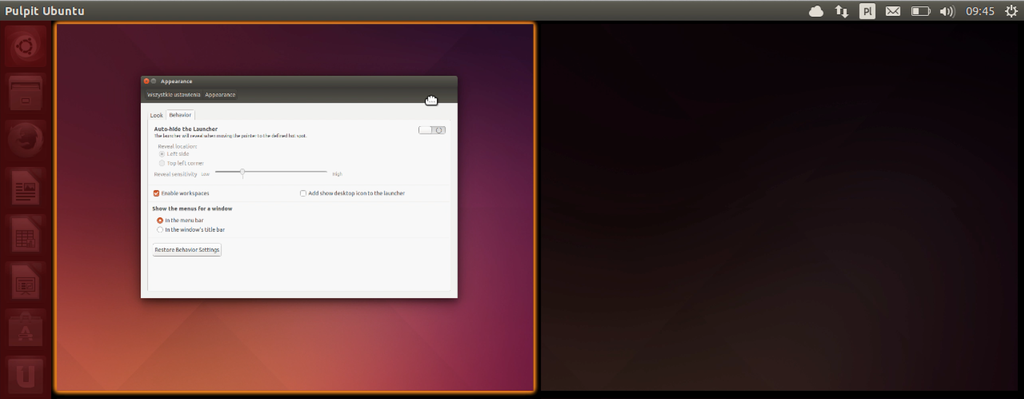
\includegraphics[width=\linewidth]{images/unity_okno_przenoszenie1.png}
\end{center}

\begin{center}
	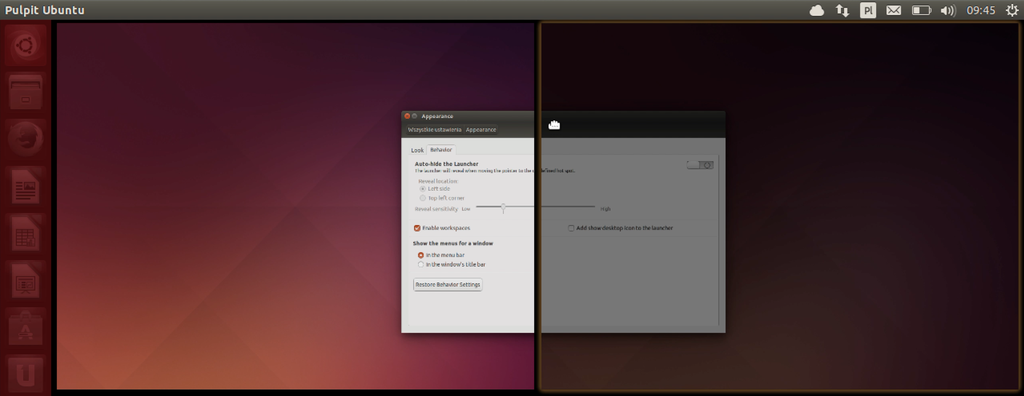
\includegraphics[width=\linewidth]{images/unity_okno_przenoszenie2.png}
\end{center}

\begin{center}
	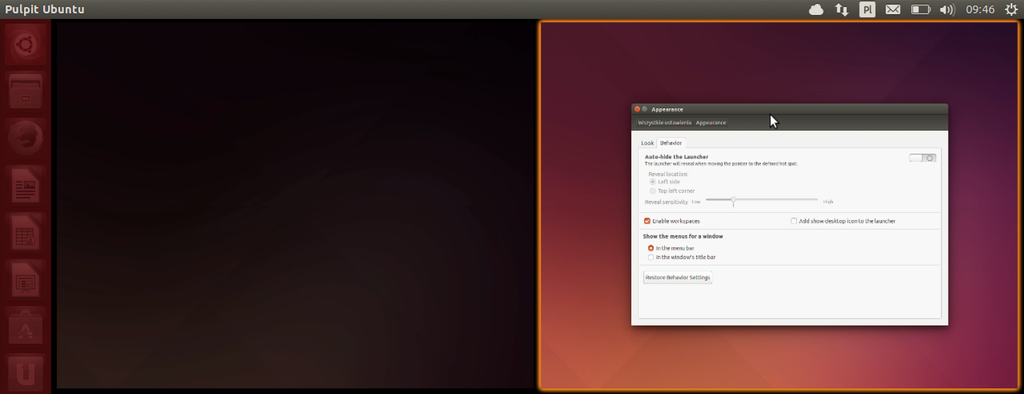
\includegraphics[width=\linewidth]{images/unity_okno_przenoszenie3.png}
\end{center}

Aby przenieść okno do innego obszaru roboczego, można również nacisnąć prawym przyciskiem myszy na pasku tytułowym otwartego okna i z menu kontekstowego wybrać którąś z dostępnych opcji:
\begin{itemize}
\item \textcolor{ubuntu_orange}{Przenieś do lewego obszaru}, gdy chcemy przenieść okno do lewego obszaru.
\item \textcolor{ubuntu_orange}{Przenieś do prawego obszaru}, gdy chcemy przenieść okno do prawego obszaru.
\item \textcolor{ubuntu_orange}{Przenieś do dolnego obszaru}, gdy chcemy przenieść okno do dolnego obszaru.
\item \textcolor{ubuntu_orange}{Przenieś do górnego obszaru}, gdy chcemy przenieść okno do górnego obszaru.
\item \textcolor{ubuntu_orange}{Przenieś do innego obszaru}, gdy chcemy wybrać, do którego konkretnie obszaru chcemy przenieść okno.
\end{itemize}

\subsubsection{Zawsze na wierzchu}
Niekiedy może zajść potrzeba, że okno jakieś aplikacji chcemy mieć zawsze widoczne na pierwszym planie pomimo tego, że aktualnie pracujemy w innym oknie. Aby utrzymać okno zawsze widoczne na pierwszym planie, należy na belce tytułowej okna nacisnąć prawym przyciskiem myszy i z menu kontekstowego, wybrać opcję \textcolor{ubuntu_orange}{Zawsze na wierzchu}.

\subsubsection{Zawsze na widocznym obszarze roboczym}
W Ubuntu dostępna jest jeszcze jedna bardzo przydatna funkcja związana z zachowaniem okiem. Gdy wykorzystujemy obszary robocze czasami może zajść potrzeba, aby okno aplikacji pojawiało się na każdym obszarze roboczym, który jest w danej chwili wykorzystywany. Aby okno pojawiało się na każdym widocznym obszarze roboczym należy na belce tytułowej okna nacisnąć prawym przyciskiem myszy i z menu kontekstowego wybrać opcję \textcolor{ubuntu_orange}{Zawsze na widocznym obszarze roboczym}.